\chapter{Języki i~metody programowania}
\PartialToc
%\startcontents[chapters]
%\printcontents[chapters]{}{1}{\section*{\contentsname}}
\section{IT1A\_W03,IT1A\_U03,IT1A\_U07}
\textbf{W~jaki sposób można obliczyć długość tekstu przekazanego jako argument w~poniższej funkcji?}
\begin{lstlisting}[language=c]
void foo(const char* txt) {
. . .
}
\end{lstlisting}
\subsection{Odpowiedź}

\begin{itemize}
\item Używając funkcji strlen z biblioteki string.h
\begin{lstlisting}[language=c]
/* Declaration */
size_t strlen(const char *str)

/* Example */
strlen(txt)
\end{lstlisting}

\item Zliczając ile znaków występuje w tekście od znaku na który wskazuje wskaźnik do znaku końca łańcucha znaków ('\textbackslash0')
\begin{lstlisting}[language=c]
int length = 0;
char c = *txt;
while(c != '\0') {
   length++;
   c = *(++txt);
}
\end{lstlisting}
\end{itemize}
  
\subsection{Wprowadzenie teoretyczne}
\textbf{Łańcuch znaków}\\
Łańuch znaków w języku C to tablica znaków której ostatni element ma wartość \textbackslash0 - null\\
Poniższe deklaracje łańcucha znaków są równoważne:
\begin{lstlisting}[language=c]
char greeting[]  = "Hello";
char greeting[6] = "Hello";
char *greeting   = "Hello";
char greeting[]  = { 'H', 'e', 'l', 'l' 'o', '\0'};
char greeting[6] = { 'H', 'e', 'l', 'l' 'o', '\0'};
\end{lstlisting}

\begin{center}
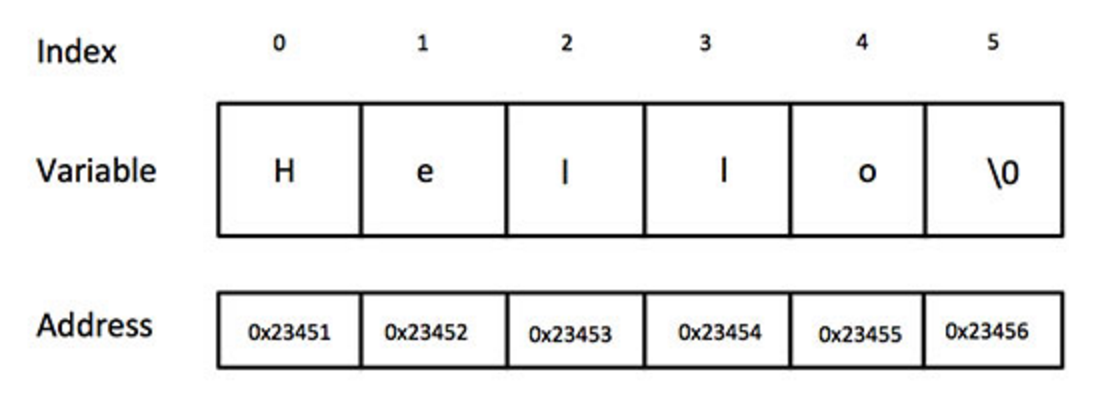
\includegraphics[width=13cm]{string_in_c}
\captionof{figure}{Łańcuchy znaków w C}
\end{center}

Istnieje biblioteka string.h która zawiera funkcja ułatwiające manipulowanie łańcuchami znaków.
\begin{lstlisting}[language=c]
strcpy(s1, s2); 
/*Copies string s2 into string s1*/

strcat(s1, s2);
/*Concatenates string s2 onto the end of string s1*/

strlen(s1);
/*Returns the length of string s1*/

strcmp(s1, s2);
/*Returns 0 if s1 and s2 are the same; less than 0 if s1<s2; greater than 0 if s1>s2*/
\end{lstlisting}

% 2 ---------------------------------------------------------------------------------------------------------------

\section{IT1A\_W03,IT1A\_U03,IT1A\_U07}dassdas

% 3 ---------------------------------------------------------------------------------------------------------------

\section{IT1A\_W03,IT1A\_U03,IT1A\_U07} 
\textbf{W jaki sposób obliczyć długość tablicy w funkcji foo()?}
\begin{lstlisting}[language=c]
void foo(double t[]){
   // dlugosc tablicy t?
}
\end{lstlisting}

\subsection{Odpowiedź}
\begin{itemize}
\item W tym wypadku nie jest możliwe obliczenie długości tablicy.\\
\end{itemize}

\subsection{Wprowadzenie teoretyczne}
Nie jest możliwe obliczenie długości tablicy posiadając jedynie wskaźnik do niej.\\
Kompilator języka C potrafi obliczyć długość tablicy jeżeli została ona zadeklarowana w tej samej metodzie w której chcemy sprawdzić długość tablicy:
\begin{lstlisting}[language=c]
int array[] = { 1, 2, 3, 4 };
int n = sizeof(array) / sizeof(array[0]);
printf("Array has %d elements\n", n); /* it should returns 4 */

foo(array);
/*...*/
void foo(int t[]){
   int n = sizeof(t) / sizeof(t[0]);
   printf("Array has %d elements\n", n); /* it shouldn't returns 4 */
}
\end{lstlisting}

% 4 ---------------------------------------------------------------------------------------------------------------

\section{Pytanie 4}dassdas

% 5 ---------------------------------------------------------------------------------------------------------------

\section{IT1A\_W03,IT1A\_U03,IT1A\_U07}
\textbf{Zakładając, ze wielkość typu char to jeden bajt, short to dwa bajty, a double to osiem bajtów, jaka jest wartość wyrażenia sizeof(x), gdzie x jest zmienną poniższego typu strukturalnego, dla standardowych ustawień kompilatora 32-bitowego?}
\begin{lstlisting}[language=c]
struct {
   char c;
   short i;
   double d;
} x;
\end{lstlisting}

\subsection{Wstęp teoretyczny}
W języku C każdy typ, oprócz char jest dopasowywany odpowiednio w przestrzeni adresowej.
\begin{itemize}
\item char może mieć początek na każdym bajcie w przestrzeni adresowej
\item short musi mieć początek na adresie parzystym
\item int lub float musi mieć początek na adresie podzielnym przez 4
\item long musi mieć początek na adresie podzielnym przez 8
\end{itemize}
\textbf{Przykład ułożenia zmiennych w pamięci: }
\begin{lstlisting}[language=c]
char *p;
char c;
int x;
\end{lstlisting}
Przestrzeń dla p zajmuje 4 bajty, zaraz po nim mamy chara 1 bajtowego. Ale rozmieszczenie 4-bajtowego x wymaga dodania luki:

\begin{lstlisting}[language=c]
char *p;      /* 4 or 8 bytes */
char c;       /* 1 byte */
char pad[3];  /* 3 bytes */
int x;        /* 4 bytes */
\end{lstlisting}
pad[3] reprezentuje fakt, że int musi zacząć się na adresie wielokrotności 4. \\\\
\textbf{Pierwszy przykład dla struktur (maszyna 64-bitowa)}
\begin{lstlisting}[language=c]
struct foo1 {
   char *p;     /* 8 bytes */
   char c;      /* 1 byte
   char pad[7]; /* 7 bytes */
   long x;      /* 8 bytes */
};
\end{lstlisting}
\textbf{Drugi przykład dla struktur}
\begin{lstlisting}[language=c]
struct MixedData  /* After compilation in 32-bit x86 machine */
{
    char Data1; /* 1 byte */
    char Padding1[1]; /* 1 byte for the following 'short' to be aligned on a 2 byte boundary
assuming that the address where structure begins is an even number */
    short Data2; /* 2 bytes */
    int Data3;  /* 4 bytes - largest structure member */
    char Data4; /* 1 byte */
    char Padding2[3]; /* 3 bytes to make total size of the structure 12 bytes */
};
\end{lstlisting}
Wydawać by się mogło, że sizeof(MixedData) = 9. Jednak nie - rozmiar struktury wynosi 12 bajtów! Do ostatniego elementu struktury dodany jest padding, dzięki któremu rozmiar struktury będzie wielokrotnością największego elementu struktury (tutaj int - 4 bajty).

\subsection{Odpowiedź na pytanie} 
sizeof(x) = 1 + padding(1) + 2 + padding(4) + 8 = 16 

% 6 ---------------------------------------------------------------------------------------------------------------

\section{Pytanie 6}dassdas

% 7 ---------------------------------------------------------------------------------------------------------------

\section{IT1A\_W03,IT1A\_U03,IT1A\_U07} 
\textbf{Przeanalizuj poniższą deklarację w języku C}
\begin{lstlisting}[language=c]
int (*x)(int, int);
\end{lstlisting}

\subsection{Odpowiedź}
\begin{itemize}
\item Deklaracja wskaźnika na funkcję przyjmującą jako parametr dwa integery\\
\end{itemize}

\subsection{Wprowadzenie teoretyczne}
\textbf{Wskaźniki na funkcje}\\
Każda funkcja tak jak i zmienna ma swoje miejsce w pamięci do którego można przypisać wskaźnik.\\
Wskaźnik na funkcje różni się od wskaźników na zmienne deklaracją:
\begin{lstlisting}[language=c]
typ_zwracanej_wartosci (*nazwa_wskaznika)(typ1 argument1, typ2 argument2, ...);
\end{lstlisting}
Przypisując nazwę funkcji bez nawiasów do wskaźnika automatycznie informujemy kompilator, że chodzi nam o adres funkcji.\\
Wskaźnika używamy tak, jak normalnej funkcji, na którą on wskazuje.\\
Przykład:
\begin{lstlisting}[language=c]
#include <stdio.h>

int suma (int lhs, int rhs){
   return lhs+rhs;
}
 
int main (){
   int (*wsk_suma)(int a, int b);
   wsk_suma = suma;
   printf("4+5=%d\n", wsk_suma(4,5));
   return 0;
}
\end{lstlisting}

% 8 ---------------------------------------------------------------------------------------------------------------
\section{IT1A\_W03,IT1A\_U03,IT1A\_U07} 
% 9 ---------------------------------------------------------------------------------------------------------------
\section{IT1A\_W03,IT1A\_U03,IT1A\_U07} 
\textbf{Które stwierdzenia dotyczące modyfikatora static w języku C/C++ są poprawne}

\begin{itemize}
\item Zmienne lokalne

Modyfikator static sprawia, że obiekt w danej funkcji jest umieszczany w tej samej pamięci, co zmienna globalna i nie jest usuwany wraz z zakończeniem funkcji.
\begin{lstlisting}[language=c]
int licznik() {
  static int a;
  a++;
  return a;
}

int main() {
  printf("Wywoluje funkcje licznik %d", licznik());  /* wypisze sie 1 */
  printf("\n...drugi raz %d", licznik());     /* wypisze sie 2 */ 
}
\end{lstlisting}

Zmienne lokalne statyczne są automatycznie inicjalizowane wartością 0.

\item Pola klasy

Statyczne pole klasy jest tworzone tylko raz, w tym samym obszarze co zmienne globalne i cały czas pamięta swoją ostatnią wartość. Jest tworzone zanim zostanie utworzony pierwszy obiekt danej klasy, zazwyczaj - tworzone są już na samym starcie programu
Pole statyczne klasy pamięta swoją wartość pomiędzy obiektami. Nie ważne z jakiego obiektu się do niego odwołasz, wartość będzie ta sama, wspólna dla wszystkich obiektów.

\item Metody

Metody statyczne - można wywołać bez podawania jakiegokolwiek obiektu. Ma to jednak swoją cenę - metody statyczne mają dostęp jedynie do innych zmiennych statycznych i metod statycznych tej klasy. 

\begin{lstlisting}[language=c]
class przyklad {
  private:
    int a, b;
    static int c;
  public:
    static void metoda() {
      c=10; 
      // b=10;     - blad! 'b' nie jest statyczne! nie ma do niego dostepu
      // this->a = 10;  - blad!! w metodach statycznych 'this' nie istnieje!!
    }
};
\end{lstlisting}
\end{itemize}

Statyczne zmienne globalne i statyczne funkcje są całkowicie niewidoczne i niedostępne dla nikogo, poza plikiem, w którym zostały zdefiniowane.


% 11 ---------------------------------------------------------------------------------------------------------------

\section{IT1A\_W03,IT1A\_U03,IT1A\_U07} 
\textbf{W jaki sposób przekazywany jest parametr do będący tablicą do funkcji w języku C?}
\begin{lstlisting}[language=c]
int main(int argc, char* argv[]){
   //...
}
\end{lstlisting}

\subsection{Odpowiedź}
\begin{itemize}
\item Na stos jest przekazywany adres pierwszego elementu tablicy\\
\end{itemize}

\subsection{Wprowadzenie teoretyczne}
Tablice są przekazywane do funkcji zawsze jako wskaźnik.\\
Zwykłe zmienne oraz obiekty(struktury) mogą być przekazywane przez wartość lub przez referencję.
\begin{itemize}
\item Przez wartość - na stos trafia kopia danej zmiennej lub obiektu.\\
Jeżeli wewnątrz struktury przekazywanej przez wartość znajduje się wskaźnik (lub tablica) to zostanie skopiowany wskaźnik. W skutek czego oryginał i kopia będą współdzielić jeden wskaźnik / tablicę. Zmieniając coś w kopii paramteru nie zmieniamy jego pierwowzoru.
\item Przez referencję - na stos trafia kopia adresu przesyłanego paramteru. Zmieniając coś w referencji, zmieniamy oryginał.
\end{itemize}

% 12 ---------------------------------------------------------------------------------------------------------------
\section{IT1A\_W03,IT1A\_U03,IT1A\_U07} 

% 13 ---------------------------------------------------------------------------------------------------------------

\section{IT1A\_W04,IT1A\_U04,IT1A\_U21} 
\textbf{Które ze stwierdzeń, odnoszących się do referencji w języku C++ są poprawne?}

\subsection{Wprowadzenie teoretyczne}
Referencja w swym działaniu przypomina wskaźniki. Różnica polega jednak na tym, że do referencji można przypisać adres tylko raz ( w momencie deklaracji ), a jej dalsze używanie niczym się nie różni od używania zwykłej zmiennej. Operacje jakie wykona się na zmiennej referencyjnej, zostaną odzwierciedlone na zmiennej zwykłej, z której pobrano adres.\\
Przykład użycia:
\begin{lstlisting}[language=c]
int i = 0;
int &ref_i = i;
cout << i;      // wypisze 0
ref_i = 1;
cout << i;      // wypisze 1
cout << ref_i;  // wypisze 1
\end{lstlisting}
Różnice między wskaźnikami i referencjami:
\begin{lstlisting}[language=c]
int a,b;
int *wsk_a = &a, *wsk_b = &b;
int &ref_a = a, &ref_b = b;
int &ref_c; // kompilator nie zezwoli na to - referencja niezainicjalizowana

wsk_b = &a; // ok
ref_b = &a; // tak sie nie da
\end{lstlisting}
W C++ można było przekazywać parametry do funkcji przez referencję w podobny sposób jak w C. W C++ jednak używa się referencji w o wiele prostszy sposób ( tak jak zwykły parametr ).

\begin{lstlisting}[language=c]
void zwieksz_c (int *i){
   ++(*i); // ta funkcja jest napisana w stylu C
}
void zwieksz_cpp (int& i){
   ++i;    // ta funkcja wykorzystuje mozliwosci C++
}

// wywolanie funkcji niczym sie nie rozni.
int i = 10;
zwieksz_c(&i);
zwieksz_cpp(&i);
\end{lstlisting}

% 14 ---------------------------------------------------------------------------------------------------------------
\section{IT1A\_W04,IT1A\_U04,IT1A\_U07,IT1A\_U21} 

% 15 ---------------------------------------------------------------------------------------------------------------
\section{IT1A\_W04,IT1A\_U04,IT1A\_U07,IT1A\_U21} 
\textbf{Przeanalizuj fragment kodu w języku C++, w którym pojawia się wywołanie operatora <<:}
\begin{lstlisting}[language=c]
A a;
std::cout<<a;
\end{lstlisting}
Która z podanych implementacji operatora << jest poprawna (przykładowy kod zostanie skompilowany i wykonany)?

\subsection{Wstęp teoretyczny}
Aby przeładować operator << musimy zdefiniować funkcję o prototypie: 
\begin{lstlisting}[language=c]
ostream& operator<<(ostream&, const Klasa&);
\end{lstlisting}
Jeśli przy wypisywaniu informacji o obiekcie potrzebny jest dostęp do prywatnych lub chronionych składowych, to funkcję tę należy też zadeklarować jako zaprzyjaźnioną wewnątrz klasy:
\begin{lstlisting}[language=c]
class Klasa {
  public:
   friend ostream& operator<<(ostream&, const Klasa&);
};
\end{lstlisting}
Przykład implementacji funkcji:
\begin{lstlisting}[language=c]
ostream& operator<<(ostream& str, const Klasa& k) {
   return str << k.nazwa << " (" << k.nazwa2 << ")";
}
\end{lstlisting}
\subsection{Odpowiedź}
Według odpowiedzi z egzaminu 2011, poprawne były odpowiedzi dwie, w których operator był w osobnej funkcji

% 16 ---------------------------------------------------------------------------------------------------------------
\section{IT1A\_W04,IT1A\_U04,IT1A\_U07,IT1A\_U21} 

% 17 ---------------------------------------------------------------------------------------------------------------
\section{IT1A\_W04,IT1A\_U04,IT1A\_U07,IT1A\_U21} 
\textbf{Klasa B przechowuje wskaźniki do obiektów klasy A w kontenerze vector standardowej biblioteki C++ (STL)}
\begin{lstlisting}[language=c]
class A{...};
class B{
   public:
   std::vector<A*> v;
   void add(A &a) { v.push_back(new A(a));}
   ~B();
}
\end{lstlisting}
\textbf{Która z implementacji destruktora jest poprawna ( kompiluje się, nie prowadzi do błędów wykonania lub wycieków pamięci)?}

\subsection{Odpowiedź}
\begin{itemize}
\item 
\begin{lstlisting}[language=c]
 B::~B(){
    for ( std::vector<A*>::iterator i = v.begin(); i != v.end(); ++i )
       delete *i; // wywolujemy delete na obiekcie, nie na wskazniku do niego!
 }
\end{lstlisting}
\end{itemize}

\subsection{Wprowadzenie teoretyczne}
Dla każdego elementu w wektorze powinien zostać, wywołany operator delete. W szczególności używanie funkcji typu std::erase czy std::remove (i ich wariantów, typu std::remove\_if), czyszczenie pojemnika, itp. same nie dają poprawnego rozwiązania – na elementach musi byd jawnie wywołany operator delete, bo żadna z takich funkcji tego sama nie robi. Jeżeli mamy do czynienia z kontenerem obiektów ( czyli nie przechowujemy danych prymitywnych np. char lub wskaźników ) to możemy wywołać funkcję std::vector<T>::clear() która wywoła na każdym obiekcie operację delete.

% 19 ---------------------------------------------------------------------------------------------------------------

\section{IT1A\_W04,IT1A\_U04,IT1A\_U07,IT1A\_U21}
\textbf{Które ze stwierdzeń odnoszących się do konstruktorów kopiujących i operatorów przypisania w języku C++ są poprawne?}

\subsection{Wprowadzenie teoretyczne}
\begin{itemize}
\item Publiczny konstruktor kopiujący oraz operator przypisania zostaną automatycznie wygenerowane przez kompilator, jeśli programista je pominie.
\item Zarówno automatycznie wygenerowany konstruktor kopiujący, jak i operator przypisania kopiują obiekty bit po bicie.
\item Inicjalizacja (tworzenie obiektu na zasadzie: X x = y;) wywołuje konstruktor kopiujący, nie operator przypisania.
\item Oprócz inicjalizacji, konstruktor kopiujący wywoływany jest gdy przekazuje się lub zwraca obiekty przez wartośd (trzeba zrobid kopię obiektu).
\item W niektórych przypadkach, jeśli kompilator jest sprytny i zrobi np. optymalizację wartości zwracanej, to konstruktor kopiujący może nie zostać wywołany przy wywołaniu funkcji zwracającej obiekt przez wartośd.
\end{itemize}

% 20 ---------------------------------------------------------------------------------------------------------------

\section{IT1A\_W04,IT1A\_U04,IT1A\_U07,IT1A\_U21}

% 21 ---------------------------------------------------------------------------------------------------------------

\section{IT1A\_W04,IT1A\_U04,IT1A\_U07,IT1A\_U21}
\textbf{W języku C++ dostep do informacji o typie obiektu w trakcie wykonania programu umożliwają następujące operatory:}

\subsection{Odpowiedź}
\begin{itemize}
\item typeid
\end{itemize}

\subsection{Wprowadzenie teoretyczne}
typeid jest funkcją która zwraca obiekt klasy std::type\_info lub wyrzucającą obiekt klasy std::bad\_typeid w przypadku gdy używamy tej funkcji z nullową wartością.\\
Przykład:
\begin{lstlisting}[language=c]
#include <iostream>
#include <typeinfo>  //for 'typeid' to work

class Person {
public:
   // ... Person members ...
   virtual ~Person() {}
};

class Employee : public Person {
   // ... Employee members ...
};

int main () {
   Person person;
   Employee employee;
   Person *ptr = &employee;
   // The string returned by typeid::name is implementation-defined
   
   std::cout << typeid(person).name() << std::endl;   // Person
   std::cout << typeid(employee).name() << std::endl; // Employee
   std::cout << typeid(ptr).name() << std::endl;      // Person * 
   std::cout << typeid(*ptr).name() << std::endl;     // Employee
}
\end{lstlisting}

% 22 ---------------------------------------------------------------------------------------------------------------

\section{IT1A\_W04,IT1A\_U04,IT1A\_U07,IT1A\_U21}
